\newcommand{\unittitle}[2]{\textbf{#1 (#2)}\newline}


\section{Unit Tests (8P)}
\subsection{10 Unit Tests (2P)}
\task{Zeigen und Beschreiben von 10 Unit-Tests und Beschreibung, was getestet wird}
\begin{enumerate}
    %% ITEM 1
    \item \unittitle{Find User by Name Test}{SqliteUserDatabaseServiceTest}
Erstelle einen neuen Nutzer mit dem Name Test und prüfe ob dieser über die findUserWithName Funktion gefunden werden kann. 
    \lstinputlisting[
    language=Java,style=codeStyle]{kapitel5_unit_tests/tests/test1.java}
    %% ITEM 2
    \item \unittitle{Update User Password Test}{SqliteUserDatabaseServiceTest}
Erstelle einen neuen Nutzer mit dem Name Test und einem Standard-Passwort. Das Passwort wird daraufhin geupdatet. Anschließend wird geprüft das neue Passwort gesetzt wurde.  
    \lstinputlisting[
    language=Java,style=codeStyle]{kapitel5_unit_tests/tests/test2.java}
    %% ITEM 3
    \item \unittitle{Get Localized Message Test}{LocalizationTest}
Prüfe ob die Übersetzungsfunktion richtig funktioniert. In diesem Test wird geprüft, ob ein existenter Language Key richtig aufgelöst werden kann.
    \lstinputlisting[
    language=Java,style=codeStyle]{kapitel5_unit_tests/tests/test3.java}
    %% ITEM 4
    \item \unittitle{Get Localized Message with Parameters}{LocalizationTest}
Prüfe ob eine Übersetzung mit Parametern gefüllt werden kann. 
    \lstinputlisting[
    language=Java,style=codeStyle]{kapitel5_unit_tests/tests/test4.java}

    %% ITEM 5
    \item \unittitle{Table Cell Tests}{HtmlDataCellTest}
Die HtmlDataCell Klasse generiert HTML Tabellen Tags für das Finanzbericht Report Feature. Es wird getestet, ob die Klasse gültige HTML-Tags ausgibt. 
    \lstinputlisting[
    language=Java,style=codeStyle]{kapitel5_unit_tests/tests/test5.java}
    %% ITEM 6
    \item \unittitle{Create and Get Transaction}{SqliteTransactionServiceTest}
Erstelle eine Zahlungstransaktion für einen Beispielnutzer und prüfe ob diese richtig gespeichert wurde. 
    \lstinputlisting[
    language=Java,style=codeStyle]{kapitel5_unit_tests/tests/test6.java}

     %% ITEM 7
    \item \unittitle{Create Transaction for Invalid User}{SqliteTransactionServiceTest}
Wenn eine Transaktion für einen nicht existenten Benutzer erzeugt wird, soll ein Fehler geworfen werden. 
    \lstinputlisting[
    language=Java,style=codeStyle]{kapitel5_unit_tests/tests/test7.java}

     %% ITEM 8
    \item \unittitle{Database Provider Test}{DatabaseProviderTest}
Prüfe ob die SqlDatabaseServiceRepository alle Services richtig erzeugt. 
    \lstinputlisting[
    language=Java,style=codeStyle]{kapitel5_unit_tests/tests/test8.java}
     %% ITEM 9
    \item \unittitle{Create and Get Bank Account}{SqliteBankAccountServiceTest}
Legt einen Bankaccount für einen Benutzer an und prüft ob die Daten richtig gespeichert wurden. 
    \lstinputlisting[
    language=Java,style=codeStyle]{kapitel5_unit_tests/tests/test9.java}
     %% ITEM 10
    \item \unittitle{Delete Bank Account}{ SqliteBankAccountServiceTest}
Erzeugt ein Konto und löscht es. 
    \lstinputlisting[
    language=Java,style=codeStyle]{kapitel5_unit_tests/tests/test10.java}
\end{enumerate}


\subsection{ATRIP: Automatic, Thorough und Professional (2P)}
\task{je Begründung/Erläuterung, wie ‘Automatic’, ‘Thorough’ und ‘Professional’ realisiert wurde – bei ‘Thorough’ zusätzlich Analyse und Bewertung zur Testabdeckung}
\begin{itemize}
    \item \textbf{Automatic}\newline 
Als Framework für die automatisierten Tests wird JUnit verwendet. Das Maven Surefire Plugin führt die Softwaretests direkt beim Kompilierungsprozess aus. 
    \item \textbf{Thorough}\newline 
Es werden Unit und Integrationstests verwendet. Da als Datenbank SQLite eingesetzt wird und die Datenbank dadurch lokal läuft, wird im Code selbst nicht zwischen Unit und Integrationstests unterschieden.  

Die Testabdeckung liegt derzeit bei lediglich 22\% und ist somit nicht besonders hoch. Auffällig ist dabei, dass der Datenbank-Layer mit einer Abdeckung von über 95\% deutlich besser getestet ist als andere Komponenten. Derzeit werden nur einzelne Befehle automatisiert getestet, was vor allem dem hohen Implementierungsaufwand geschuldet ist. Dieser entsteht insbesondere dadurch, dass für die Tests Datenbank-Services gemockt werden müssen.
 
    \item \textbf{Professional}\newline 
Unsere automatisierten Softwaretests sind professionell, da diese einer klaren Struktur folgen: Die zu einer Klasse gehörenden Tests befinden sich immer in der entsprechenden Datei Namens \textit{[domain.package.Example]Test}. Die Tests sind sinnvoll benannt und testen immer nur einen Pfad einer Funktionalität. Der Testcode folgt den allgemeinen Regeln zu Clean Code.
\end{itemize}


\subsection{Fakes und Mocks (4P)}
\task{Analyse und Begründung des Einsatzes von 2 Fake/Mock-Objekten (die Fake/Mocks sind ohne 
Dritthersteller-Bibliothek/Framework zu implementieren); zusätzlich jeweils UML Diagramm mit Beziehungen zwischen Mock, zu mockender Klasse und Aufrufer des Mocks}

\subsubsection*{CategoryService Mock}
\lstinputlisting[language=Java,style=codeStyle]{kapitel5_unit_tests/mock/mock1.java}
In diesem Unit Test wird der Create Category Command getestet. Um nicht die Datenbanklogik testen zu müssen wird ein Mock Objekt eingesetzt. Der MockedCategoryService ist eine Implementierung des CategoryService Interface.  

\begin{figure}[htbp]
    \centering
    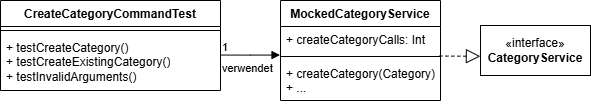
\includegraphics[width=\linewidth]{kapitel5_unit_tests/mock1.drawio.png}
\end{figure}
\newpage
\subsubsection*{BankAccountService Mock}
\lstinputlisting[language=Java,style=codeStyle]{kapitel5_unit_tests/mock/mock2.java}
In den Tests der Klasse \textit{SqliteTransactionServiceTest} wird der TransactionService getestet. Dieser benötigt als Abhängigkeit einen BankAccount Service. Da dieser nicht mitgetestet werden soll wird der BankAccount Service gemockt.
\begin{figure}[htbp]
    \centering
    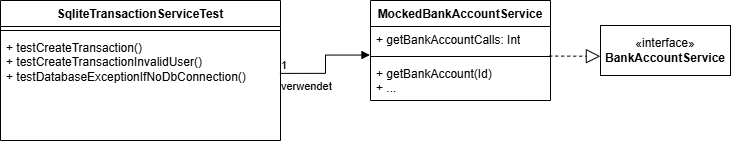
\includegraphics[width=\linewidth]{kapitel5_unit_tests/mock2.drawio.png}
\end{figure}